\section{The solution}
We want to decompose 
\begin{equation}
    U_{\text{Heis3}}(t) = \exp\left[-it \sum_{\langle ij \rangle}^{N=3} \left(\sigma_x^{(i)}\sigma_x^{(j)} + \sigma_y^{(i)}\sigma_y^{(j)} + \sigma_z^{(i)}\sigma_z^{(j)}\right) \right]
    \end{equation}
into single and two-qubit gates.

Since the Pauli operators do not commute with each other~\cite{Shankar} the exponential $U_{\text{Heis3}}(t)$ cannot be split into a product of simpler exponentials.

However, we can approximate $U_{\text{Heis3}}(t)$ as a product of simpler exponentials through Trotterization. Consider a subsystem of 2 spin-1/2 particles within the larger 3 spin system. The Hamiltonian on spins $i$ and $j$ ($i,j \in \{0,1,2\}$) would be $H^{(i,j)}_{\text{Heis2}} = \sigma_x^{(i)}\sigma_x^{(j)} + \sigma_y^{(i)}\sigma_y^{(j)} + \sigma_z^{(i)}\sigma_z^{(j)}$. Rewriting $U_{\text{Heis3}}(t)$ in terms of the two possible subsystems within the total $N=3$ system you will simulate,

\begin{equation}
U_{\text{Heis3}}(t) = \exp\left[-i t \left(H^{(0,1)}_{\text{Heis2}} + H^{(1,2)}_{\text{Heis2}} \right)\right].
\end{equation}

$H^{(0,1)}_{\text{Heis2}}$ and $H^{(1,2)}_{\text{Heis2}}$ do not commute, so
\begin{equation}
 U_{\text{Heis3}}(t) \neq \exp\left(-i t H^{(0,1)}_{\text{Heis2}}\right) \exp\left(-i t H^{(1,2)}_{\text{Heis2}} \right)
\end{equation}. 
 
 But, this product decomposition can be approximated with Trotterization which says $U_{\text{Heis3}}(t)$ is approximately a short evolution of $H^{(0,1)}_{\text{Heis2}}$ (time = $t/n$) and followed by a short evolution of $H^{(1,2)}_{\text{Heis2}}$ (time = $t/n$) repeated $n$ times


\begin{align}
U_{\text{Heis3}}(t) &= \exp\left[-i t \left(H^{(0,1)}_{\text{Heis2}} + H^{(1,2)}_{\text{Heis2}} \right)\right] \\
U_{\text{Heis3}}(t) &\approx \left[\exp\left(\dfrac{-it}{n}H^{(0,1)}_{\text{Heis2}}\right) \exp\left(\dfrac{-it}{n}H^{(1,2)}_{\text{Heis2}} \right)\right]^n.
\end{align}


$n$ is the number of Trotter steps, and as $n$ increases, the approximation should becomes more accurate but as we have already anticipated experimentally this not seems to be the case.

But now we have a state of the art solution for decomposing \text{Heis2} into quantum gates~\cite{s1} \cite{s2} and this is shown in figure~\ref{fig:solution}, we can then implement this decomposition of \text{Heis2} into our decomposition of \text{Heis3}.

In the decomposition of Heis2 we have:

\begin{equation}
    R X(\theta)=\exp \left(-i \frac{\theta}{2} X\right)=\left(\begin{array}{cc}
        \cos \frac{\theta}{2} & -i \sin \frac{\theta}{2} \\
        -i \sin \frac{\theta}{2} & \cos \frac{\theta}{2}
        \end{array}\right)
\end{equation}

and 
\begin{equation}
    R Z(\lambda)=\exp \left(-i \frac{\lambda}{2} Z\right)=\left(\begin{array}{cc}
        e^{-i \frac{\lambda}{2}} & 0 \\
        0 & e^{i \frac{\lambda}{2}}
        \end{array}\right).
\end{equation}

Those are not native gates but as already said they can be implemented as Jakarta has a universal set of quantum gates, and we can change the phase factor directly without the need of using Pulse.
\begin{figure}[htb]
    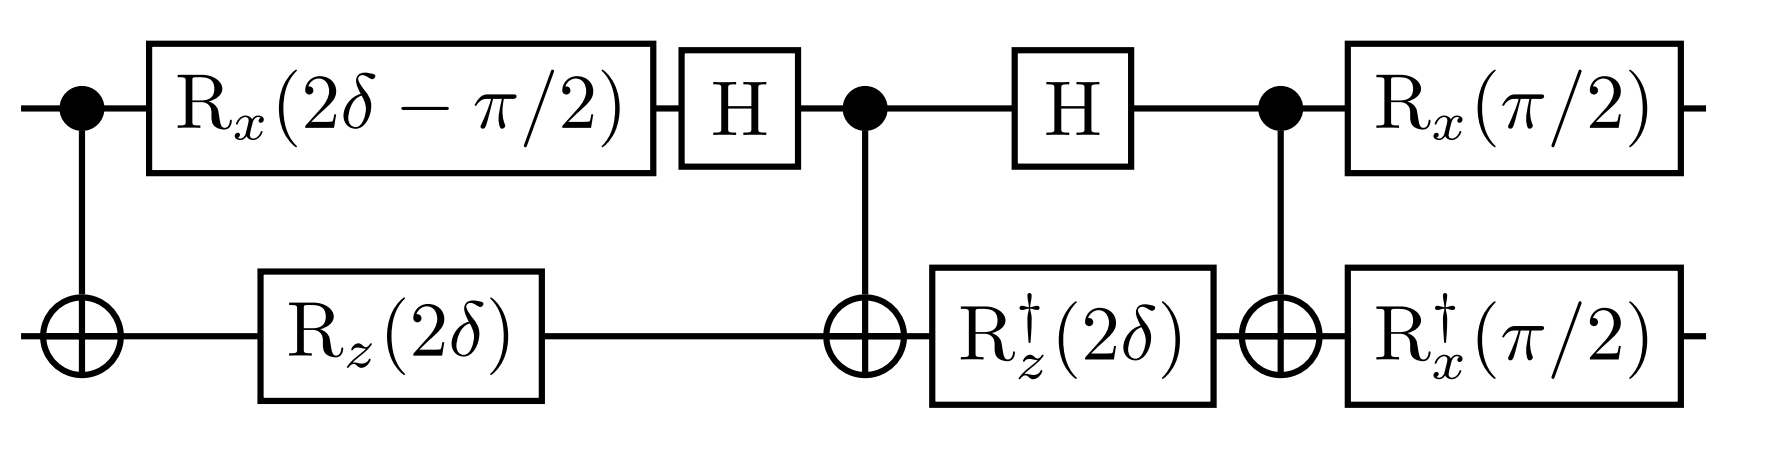
\includegraphics[width = 1.2\textwidth]{circuit.png}
    \centering
    \caption{Heis2 decomposition}
    \label{fig:solution}
\end{figure}


At the end our circuit is represented in figure~\ref{fig:circuit} where we can see the 7 qubits, the 4 trotterization steps and the measure at the end. The circuit of~\ref{fig:solution} is contained in each trotterization step. 
\begin{figure}[htb]
    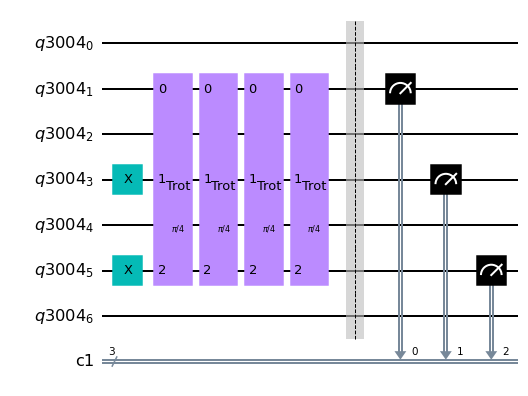
\includegraphics[width = 1.2\textwidth]{output1.png}
    \centering
    \caption{Circuit overview}
    \label{fig:circuit}
\end{figure}

Finally, those are the results:
\begin{description}
    \item[Noisy simulation: ]0.4405 ± 0.0011 (N=4)
    \item[Real device: ]0.3108 ± 0.0034 (N=4)
    \end{description}

    You may ask why there were not tried more complicated decomposition, the reason is that at the end reducing the original Hamiltonian to Hamiltonians with already recognized state of the art decomposition resulted to be the strategy that provided the better results, as completely raw decomposition directly to gates resulted in significantly weaker results.

    In addition to that the least number of trotterization steps as the problem required were used. This is because, contrary to what Lie's formula presented in chapter~\ref{chap:2} seems to suggests, experimentally it was very clear that augmenting trotterization steps significantly reduced state tomography results, probably because no noise suppression techniques were used in order to deal with the the fact that the circuit increases with more Trotterization steps.
